%!TEX program = xelatex
\let\stop\empty

\documentclass[12pt,a4paper]{exam-zh}

\usepackage{xeCJK}
\setCJKmainfont{Noto Serif CJK SC}
\usepackage{geometry}
\usepackage{array}
\usepackage{tikz}
\usetikzlibrary{calc,angles,quotes}
\usepackage{amsmath}
\usepackage{wrapfig}
\usepackage{adjustbox}
\usepackage{enumitem}
\usepackage{fancyhdr}


\usepackage{scalerel}
\providecommand{\wideparen}[1]{\overset{\frown}{#1}}
\def\mcirc{\mathbin{\scalerel*{\circ}{j}}}
\def\msquare{\mathord{\scalerel*{\Box}{gX}}}
\geometry{margin=2cm}

% \AtBeginDocument{\zihao{4}}
% ----------- 调整 exam -----------


% --- 全局样式定义 ---
% 定义选择题环境：题号 1. 2.，选项 A. B. C. D. 粗体，且保留 1.5em 间距
\examsetup{
    page = {
    size = a4paper,           % 设定纸张大小 [4]
    foot-content = { - ; - }  % 页脚显示为 -1-, -2- 格式 [3]
  },
    choices = {
    label-pos = top-left,
    column-sep = 1em,
    label-pos = auto,
    label-sep = 0.5em,
    max-columns = 4
    },
  question = {
    top-sep    = 1em, % 调整题目上方的垂直距离（默认值为 .5em plus .5em minus .2em）
    bottom-sep = 1em  % 调整题目下方的垂直距离（默认值为 .5em plus .5em minus .2em）
  },
    paren = {
    show-paren = false  % 设置为 false 则不显示括号 [3, 4]
  },
    choices = {
    label = \textbf{\Alph*}
  }, 
    solution = {
    show-solution = show-move, % 答案自动移动到卷末
    label-content = {参考答案},  % 答案区的标题文字
    show-qed = true            % 在解答末尾显示结束符号 ◻ 
  }
}

% ==========================
% 卷面变量设置（只需改这里）
% ==========================
% ==========================
% 卷面变量设置（只需改这里）
% ==========================
\newcommand{\paperlevel}{初中二}
\newcommand{\papersubject}{数学 试卷一}
\newcommand{\schoolname}{金宝培元独立中学}
\newcommand{\examname}{八月考}
\newcommand{\classinfo}{J2(H / I/ F)}
\newcommand{\examdate}{5-8-2026}
\newcommand{\examtime}{10:15-11:00}
\newcommand{\questiontotal}{20}
\newcommand{\paperpercentage}{40\%}
\newcommand{\setterteacher}{蔡杰庆师}
\newcommand{\reviewteacher}{谢明政师}
\newcommand{\auditteacher}{雷泳健师}

\makeatletter
\newcounter{answerkeyquestion}
\let\answerkeytotal\questiontotal
\let\originalparen\paren
\newcommand{\answerkeyitems}{}
\newcommand{\addanswerkeyitem}[2]{%
  \pgfmathtruncatemacro{\row}{ifthenelse(#1<=\cols,0,1)}%
  \pgfmathtruncatemacro{\col}{mod(#1-1,\cols)}%
  \pgfmathsetlengthmacro{\x}{\col*\boxw}%
  \pgfmathsetlengthmacro{\y}{-\row*\boxh}%
  \draw (\x,\y) rectangle ++(\boxw,\boxh);%
  \node[anchor=north west] at (\x+\offset,\y+\boxh-\offset) {\textbf{#1.}};%
  \node at (\x+0.6*\boxw,\y+0.45*\boxh) {\Large\textbf{#2}};%
}
\renewcommand{\paren}[1][]{%
  \originalparen[#1]%
  \edef\answerkeytemp{#1}%
  \ifx\answerkeytemp\@empty\else
    \stepcounter{answerkeyquestion}%
    \begingroup
      \edef\x{\endgroup
        \noexpand\g@addto@macro\noexpand\answerkeyitems{\noexpand\addanswerkeyitem{\theanswerkeyquestion}{#1}}}%
    \x
  \fi
}
\makeatother

\begin{document}

% ==========================
% 三栏标题区
% ==========================
\noindent
\begin{tabular*}{\textwidth}{@{\extracolsep{\fill}} p{0.3\textwidth} p{0.35\textwidth} p{0.3\textwidth}}

\raggedright
\textbf{\paperlevel}\\[0.2em]
\textbf{}{\papersubject}\\[0.4em]
姓名：\underline{\hspace{3cm}} &

\centering
\textbf{\schoolname}\\[0.2em]
\textbf{\examname}\\[0.4em]
班级：\classinfo&

\raggedright
日期：\examdate\\[0.2em]
时间：\examtime\\[0.4em]
得分：\underline{\hspace{2.5cm}} \\

\end{tabular*}

\begin{flushleft}
考生须知： 
选出正确的答案，用蓝或黑色的原子笔将答案的相应选项字母填入本页特备作答栏。
\end{flushleft}

% =========================
% 答题栏
% =========================
\begin{flushleft}
\textbf{特备答题栏:}
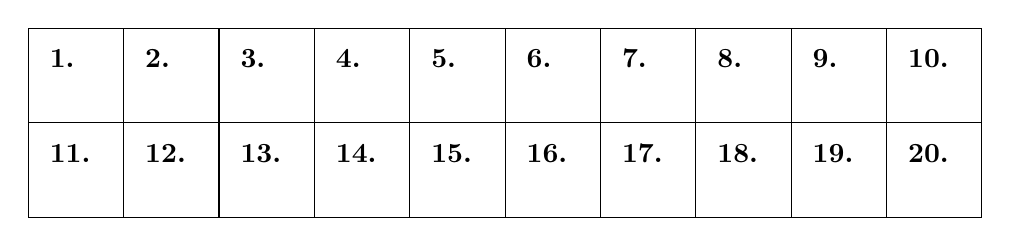
\begin{tikzpicture}
  % ---- 根据题数自动设置：16题为 8×2，20题为 10×2 ----
  \pgfmathtruncatemacro{\cols}{ifthenelse(\answerkeytotal<=16,8,10)}
  \pgfmathsetlengthmacro{\boxw}{(\linewidth-0.4pt)/\cols}
  \pgfmathsetlengthmacro{\boxh}{1.2cm}
  \pgfmathsetlengthmacro{\offset}{0.15cm}

  \foreach \num in {1,...,\answerkeytotal} {
    \pgfmathtruncatemacro{\row}{ifthenelse(\num<=\cols,0,1)}
    \pgfmathtruncatemacro{\col}{mod(\num-1,\cols)}
    \pgfmathsetlengthmacro{\x}{\col*\boxw}
    \pgfmathsetlengthmacro{\y}{-\row*\boxh}
    \draw (\x,\y) rectangle ++(\boxw,\boxh);
    \node[anchor=north west] at (\x+\offset,\y+\boxh-\offset) {\textbf{\num.}};
  }
\end{tikzpicture}

\end{flushleft}

%region 范围：初一（Form 1）基础几何 | 考点：平行四边形面积公式（底×高） | 难度：基础
\begin{question}
    如下图所示，平行四边形 $ABCD$ 中，底边 $AB = 8\text{ cm}$，一腰 $AD = 6\text{ cm}$，$AB$ 边上的高为 $5\text{ cm}$，则该平行四边形的面积为 
    \paren[C]


    \begin{center}
    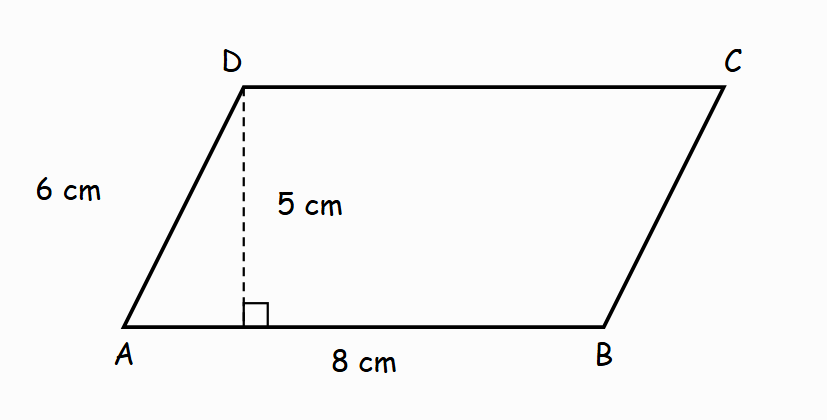
\includegraphics[width=0.5\textwidth]{AUG_J2_PAPER1/image.png}
    % \begin{tikzpicture}[scale=0.55]
    %     \coordinate (A) at (0,0);
    %     \coordinate (B) at (8,0);
    %     \coordinate (C) at (9.5,3);
    %     \coordinate (D) at (1.5,3);
    %     \coordinate (E) at (1.5,0);

    %     \draw[thick] (A) -- (B) -- (C) -- (D) -- cycle;
    %     \draw[dashed] (D) -- (E);
    %     \draw (1.5,0.3) -- (1.8,0.3) -- (1.8,0);

    %     \node[below] at ($(A)!0.5!(B)$) {$8\text{ cm}$};
    %     \node[left]  at ($(A)!0.5!(D)$) {$6\text{ cm}$};
    %     \node[right] at ($(D)!0.5!(E)$) {$5\text{ cm}$};

    %     \node[below left]  at (A) {$A$};
    %     \node[below right] at (B) {$B$};
    %     \node[above right] at (C) {$C$};
    %     \node[above left]  at (D) {$D$};
    % \end{tikzpicture}
    \end{center}

    \begin{choices}
        \item $20\text{ cm}^2$
        \item $28\text{ cm}^2$
        \item $40\text{ cm}^2$
        \item $48\text{ cm}^2$
    \end{choices}
\end{question}

\begin{solution}
    求平行四边形 $ABCD$ 的面积，已知 $AB=8\text{ cm}$，$AB$ 边上的高为 $5\text{ cm}$。\\
    平行四边形面积公式为「底 $\times$ 高」，须用底边对应的高，而非腰长。
    \[
        S = AB \times h = 8 \times 5 = 40 \text{ (cm}^2\text{)}
    \]
    故选 C。
\end{solution}
%endregion

%region 范围：初中/高中几何 - 四边形性质 | 考点：对角线判别四边形类型 | 难度：基础
\begin{question}
    在凸四边形中，若对角线互相垂直且互相平分，则该四边形必为下列何种图形？ \paren[C]
    \begin{choices}
        \item 平行四边形
        \item 长方形
        \item 菱形
        \item 正方形
    \end{choices}
\end{question}

\begin{solution}
    判断对角线互相垂直且互相平分的凸四边形必为何种图形。\\
    对角线互相平分 $\Rightarrow$ 平行四边形；再加垂直条件 $\Rightarrow$ 邻边相等，即菱形。
    \[
        \text{对角线互相平分} \implies \text{平行四边形；再加垂直} \implies \text{四边相等} \implies \text{菱形}
    \]
    故选 C。
\end{solution}
%endregion

%region 范围：初中几何 - 多边形内角和 | 考点：内角和公式逆用求边数 | 难度：基础
\begin{question}
    已知一个凸多边形的内角和为 $1620°$，求该多边形的边数。 \paren[C]
    \begin{choices}
        \item $9$
        \item $10$
        \item $11$
        \item $12$
    \end{choices}
\end{question}

\begin{solution}
    已知凸多边形内角和为 $1620°$，求边数。\\
    代入多边形内角和公式 $(n-2)\times180°$ 解出 $n$。
    \begin{align*}
        (n-2) \times 180° &= 1620° \\
        n-2 &= 9 \\
        n &= 11
    \end{align*}
    故选 C。
\end{solution}
%endregion

% 范围：初中几何 - 正多边形 | 考点：外角和恒为360°、正多边形边数求解 | 难度：基础
%region 范围：初中几何 - 正多边形 | 考点：外角和恒为360°、正多边形边数求解 | 难度：基础
\begin{question}
    已知一个正多边形的每一个外角为 $24°$，求该正多边形的边数。 \paren[C]
    \begin{choices}
        \item $12$
        \item $13$
        \item $15$
        \item $18$
    \end{choices}
\end{question}

\begin{solution}
    已知正多边形每个外角为 $24°$，求边数。\\
    凸多边形外角和恒为 $360°$，用 $360°$ 除以每个外角度数即得边数。
    \[
        n = \frac{360°}{24°} = 15
    \]
    故选 C。
\end{solution}
%endregion

\newpage 


%region 范围：初一（Form 1）基础几何 | 考点：平行四边形与三角形面积公式的综合运用 | 难度：中等
\begin{question}
    如下图所示，梯形 $ABCD$ 由三角形 $ADE$ 与平行四边形 $EBCD$ 拼接而成，其中 $E$ 为 $AB$ 上一点。已知 $AE = 4\text{ cm}$，平行四边形 $EBCD$ 的底边 $EB = 6\text{ cm}$，其面积为 $30\text{ cm}^2$，则梯形 $ABCD$ 的面积为 \paren[B]

    \begin{center}
    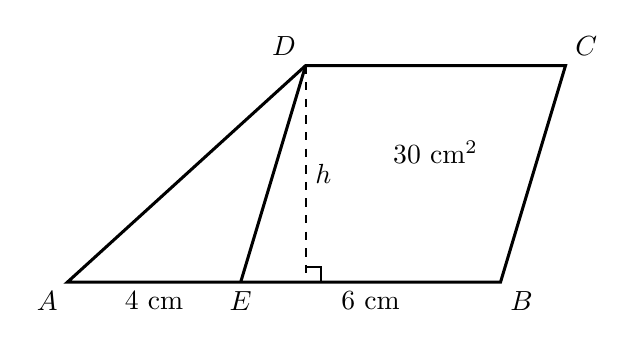
\begin{tikzpicture}[scale=0.55, every node/.style={font=\normalsize}]
        \coordinate (A) at (0,0);
        \coordinate (E) at (4,0);
        \coordinate (B) at (10,0);
        \coordinate (D) at (5.5,5);
        \coordinate (C) at (11.5,5);
        \coordinate (F) at (5.5,0);

        \draw[line width=1.1pt] (A) -- (B) -- (C) -- (D) -- cycle;
        \draw[line width=1.1pt] (E) -- (D);
        \draw[line width=0.8pt, dashed] (D) -- (F);
        \draw[line width=0.8pt] (5.5,0.35) -- (5.85,0.35) -- (5.85,0);

        \node[below] at ($(A)!0.5!(E)$) {$4\text{ cm}$};
        \node[below] at ($(E)!0.5!(B)$) {$6\text{ cm}$};
        \node at (8.5,3) {$30\text{ cm}^2$};
        \node[right] at (5.5,2.5) {$h$};

        \node[below left] at (A) {$A$};
        \node[below] at (E) {$E$};
        \node[below right] at (B) {$B$};
        \node[above right] at (C) {$C$};
        \node[above left] at (D) {$D$};
    \end{tikzpicture}
    \end{center}

    \begin{choices}
        \item $34\text{ cm}^2$
        \item $40\text{ cm}^2$
        \item $45\text{ cm}^2$
        \item $50\text{ cm}^2$
    \end{choices}
\end{question}

\begin{solution}
    求梯形 $ABCD$ 的面积，已知 $AE=4\text{ cm}$，平行四边形 $EBCD$ 底边 $EB=6\text{ cm}$，面积 $30\text{ cm}^2$。\\
    先由平行四边形面积公式求出公共高 $h$，再用三角形面积公式求 $\triangle ADE$，两者相加。
    \begin{align*}
        h &= \frac{S_{EBCD}}{EB} = \frac{30}{6} = 5 \\
        S_{ADE} &= \frac{1}{2} \times AE \times h = \frac{1}{2} \times 4 \times 5 = 10 \\
        S_{ABCD} &= S_{ADE} + S_{EBCD} = 10 + 30 = 40
    \end{align*}
    故选 B。
\end{solution}
%endregion


%region 范围：初中几何 | 考点：平行线性质、Z字型/拐点模型角度传递 | 难度：困难
\begin{question}
    如下图所示，已知AE//CD， BC//ED。求 $\angle x + \angle y$ 的度数。 \paren[C]
    
    \begin{center}
    \usetikzlibrary{decorations.markings, arrows.meta, quotes, angles, calc}
    \tikzset{
        mid arrow/.style={postaction={decorate,decoration={
            markings, mark=at position .6 with {\arrow[scale=1.2]{Latex}}
        }}},
        mid double arrow/.style={postaction={decorate,decoration={
            markings,
            mark=at position .53 with {\arrow[scale=1.2]{Latex}},
            mark=at position .63 with {\arrow[scale=1.2]{Latex}}
        }}}
    }
    \begin{tikzpicture}[scale=1]
        % 基准点
        \coordinate (A) at (0, 3.5);
        \coordinate (B) at ([shift={(-45:2.5)}]A);
        \coordinate (C) at ([shift={(43:3)}]B);
        \coordinate (E) at (0, -2);
        \coordinate (D) at (intersection of C--{[shift={(0,-5)}]C} and E--{[shift={(43:6)}]E});
        
        % 绘制左侧双箭头平行线
        \draw[thick] (0, 5) -- (A) -- (E) -- (0, -3.5);
        \draw[thick, mid double arrow] (0, 2) -- (0, -0.5);

        % 绘制右侧双箭头平行线 CD
        \draw[thick, mid double arrow] (C) -- (D);
        
        % 绘制单箭头平行线 BC 和 ED
        \draw[thick, mid arrow] (B) -- (C);
        \draw[thick, mid arrow] (E) -- (D);
        
        % 绘制连接线 AB
        \draw[thick] (A) -- (B);

        % 标注每一个点的字母
        \fill (A) circle (1.5pt) node[left=2pt] {$A$};
        \fill (B) circle (1.5pt) node[above=2pt] {$B$};
        \fill (C) circle (1.5pt) node[right=2pt] {$C$};
        \fill (D) circle (1.5pt) node[right=2pt] {$D$};
        \fill (E) circle (1.5pt) node[left=2pt] {$E$};

        % 统一使用 angle eccentricity=1.4 标注角度
        \coordinate (A_up) at (0, 4.5);
        \pic[draw, thick, angle radius=0.6cm, "$135^\circ$", angle eccentricity=1.8] {angle=B--A--A_up};
        \pic[draw, thick, angle radius=0.6cm, "$268^\circ$", angle eccentricity=1.4] {angle=A--B--C};
        \pic[draw, thick, angle radius=0.7cm, "$y$", angle eccentricity=1.4] {angle=B--C--D};
        \coordinate (E_up) at (0, -1);
        \pic[draw, thick, angle radius=0.7cm, "$x$", angle eccentricity=1.4] {angle=D--E--E_up};

    \end{tikzpicture}
    \end{center}

    \begin{choices}
        \item $86^\circ$
        \item $90^\circ$
        \item $94^\circ$
        \item $104^\circ$
    \end{choices}
\end{question}

\begin{solution}
    已知 $AE \parallel CD$，$BC \parallel ED$，拐点 $B$ 处反射角 $268°$，求 $\angle x + \angle y$。\\
    过拐点 $B$ 作辅助线 $BF \parallel AE$，借助同旁内角互补与内错角相等逐步传递角度。
    \begin{align*}
        \angle ABC &= 360°-268° = 92° \\
        \angle ABF &= 180°-135° = 45° \quad (BF\parallel AE\text{，同旁内角互补}) \\
        \angle FBC &= 92°-45° = 47° \\
        \angle y &= \angle FBC = 47° \quad (BF\parallel CD\text{，内错角相等}) \\
        \angle x &= \angle y = 47° \quad (BC\parallel ED\text{ 且 } AE\parallel CD) \\
        \angle x + \angle y &= 47°+47° = 94°
    \end{align*}
    故选 C。
\end{solution}
%endregion



\newpage

%region 范围：初中几何 | 考点：多边形内角和、外角定理、飞镖模型 | 难度：中等
\begin{question}
    如下图所示，下列哪项满足a,c,b,d之间的关系？ \paren[A]
    
    \begin{center}
    \usetikzlibrary{quotes, angles, calc}
    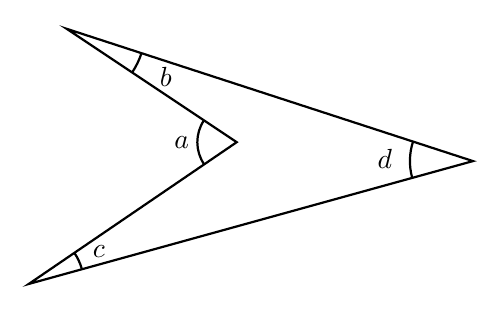
\begin{tikzpicture}[scale=1.2]
        % 定义顶点坐标
        \coordinate (A) at (0,0);       % 凹顶点
        \coordinate (B) at (-1.8, 1.2); % 左上顶点
        \coordinate (C) at (-2.2, -1.5);% 左下顶点
        \coordinate (D) at (2.5, -0.2); % 右侧顶点

        % 绘制四边形边界
        \draw[thick] (B) -- (A) -- (C) -- (D) -- cycle;

        % 标注角度 (统一使用 angle eccentricity=1.4)
        \pic[draw, thick, angle radius=0.5cm, "$a$", angle eccentricity=1.4] {angle=B--A--C};
        \pic[draw, thick, angle radius=1.0cm, "$b$", angle eccentricity=1.4] {angle=A--B--D};
        \pic[draw, thick, angle radius=0.7cm, "$c$", angle eccentricity=1.4] {angle=D--C--A};
        \pic[draw, thick, angle radius=0.8cm, "$d$", angle eccentricity=1.4] {angle=B--D--C};
    \end{tikzpicture}
    \end{center}

    \begin{choices}
        \item $a = b + c + d$
        \item $a + b + c + d = 360^\circ$
        \item $a = b + c - d$
        \item $a + b + c + d = 180^\circ$
    \end{choices}
\end{question}

\begin{solution}
    判断"飞镖模型"四边形中 $a,b,c,d$ 之间的关系。\\
    连接 $D$ 与凹顶点 $A$ 并延长至 $E$，构造两个三角形，用外角定理（外角等于不相邻两内角之和）求 $a$。
    \begin{center}
    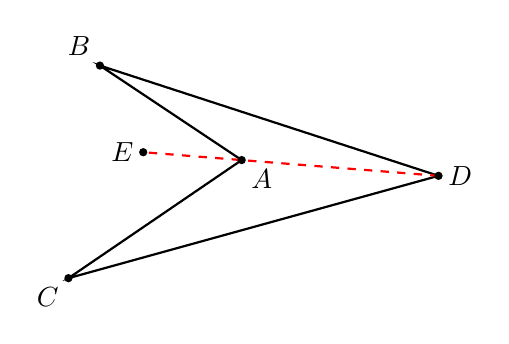
\begin{tikzpicture}[scale=1]
        \coordinate (A) at (0,0);
        \coordinate (B) at (-1.8, 1.2);
        \coordinate (C) at (-2.2, -1.5);
        \coordinate (D) at (2.5, -0.2);
        
        \draw[thick] (B) -- (A) -- (C) -- (D) -- cycle;
        
        % 辅助线
        \coordinate (E) at ($(D)!1.5!(A)$);
        \draw[dashed, red, thick] (D) -- (E);

        % 辅助点标注
        \fill (A) circle (1.5pt) node[below right] {$A$};
        \fill (B) circle (1.5pt) node[above left] {$B$};
        \fill (C) circle (1.5pt) node[below left] {$C$};
        \fill (D) circle (1.5pt) node[right] {$D$};
        \fill (E) circle (1.5pt) node[left] {$E$};
    \end{tikzpicture}
    \end{center}
    \begin{align*}
        \angle BAE &= \angle B + \angle BDA \quad (\triangle ABD \text{ 外角}) \\
        \angle CAE &= \angle C + \angle CDA \quad (\triangle ACD \text{ 外角}) \\
        a = \angle BAC = \angle BAE + \angle CAE &= \angle B + \angle C + \angle D = b+c+d
    \end{align*}
    故选 A。
\end{solution}
%endregion


%region 范围：初中几何 | 考点：平行线性质、三角形内角和、多边形角度计算 | 难度：中等
\begin{question}
    如下图所示，在梯形 $ABCD$ 中，$AD \parallel BC$。已知 $\angle BAD = 115^\circ$，$\angle BCD = 65^\circ$。连接对角线 $BD$，若 $\angle ABD = 45^\circ$，则 $\angle CDB$ 的度数为 \paren[C]
    
    \begin{center}
    \usetikzlibrary{quotes, angles, calc}
    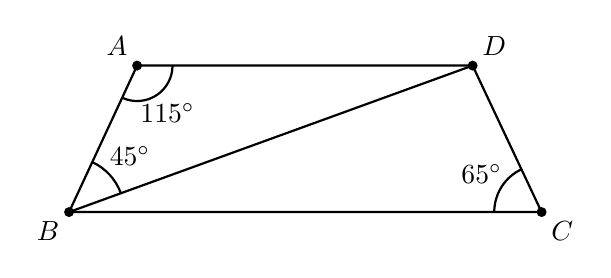
\begin{tikzpicture}[scale=1.2]
        % 根据真实角度计算的精确坐标
        % BC 放在 x 轴上，B 为原点 (0,0)
        \coordinate (B) at (0,0);
        \coordinate (C) at (5,0);
        
        % 角度 ABC = 180 - 115 = 65度。角度 DBC = 65 - 45 = 20度。
        % A 点位于 65 度的射线上，D 点位于 20 度的射线上，且 AD 平行于 BC (y坐标相同)
        % 通过几何计算得出 A 和 D 的近似坐标以保证按比例作图
        \coordinate (A) at (0.72, 1.55);
        \coordinate (D) at (4.27, 1.55);

        % 绘制梯形及对角线
        \draw[thick] (A) -- (B) -- (C) -- (D) -- cycle;
        \draw[thick] (B) -- (D);

        % 顶点标注
        \fill (A) circle (1.5pt) node[above left] {$A$};
        \fill (B) circle (1.5pt) node[below left] {$B$};
        \fill (C) circle (1.5pt) node[below right] {$C$};
        \fill (D) circle (1.5pt) node[above right] {$D$};

        % 角度标注 (统一使用 angle eccentricity=1.4)
        \pic[draw, thick, angle radius=0.45cm, "$115^\circ$", angle eccentricity=1.6] {angle=B--A--D};
        \pic[draw, thick, angle radius=0.6cm, "$65^\circ$", angle eccentricity=1.5] {angle=D--C--B};
        \pic[draw, thick, angle radius=0.7cm, "$45^\circ$", angle eccentricity=1.5] {angle=D--B--A};
    \end{tikzpicture}
    \end{center}

    \begin{choices}
        \item $45^\circ$
        \item $50^\circ$
        \item $95^\circ$
        \item $115^\circ$
    \end{choices}
\end{question}

\begin{solution}
    梯形 $ABCD$ 中 $AD\parallel BC$，$\angle BAD=115°$，$\angle BCD=65°$，$\angle ABD=45°$，求 $\angle CDB$。\\
    先由同旁内角互补求 $\angle ABC$，再求 $\angle DBC$，最后在 $\triangle BCD$ 中用内角和求解。
    \begin{align*}
        \angle ABC &= 180°-115° = 65° \quad (AD\parallel BC\text{，同旁内角互补}) \\
        \angle DBC &= \angle ABC - \angle ABD = 65°-45° = 20° \\
        \angle CDB &= 180° - \angle BCD - \angle DBC = 180°-65°-20° = 95°
    \end{align*}
    故选 C。
\end{solution}
%endregion

% 范围：小学数学/初等几何 | 考点：图形面积计算与面积单位（平方千米）换算 | 难度：中等
\begin{question}
    如下图所示，某城市规划了一块矩形硬化场地用于建设大型市民广场。已知该矩形场地的长为 $500 \, \mathrm{m}$，宽为 $400 \, \mathrm{m}$。请问这块场地的面积是?\paren[A]
    
    \begin{center}
    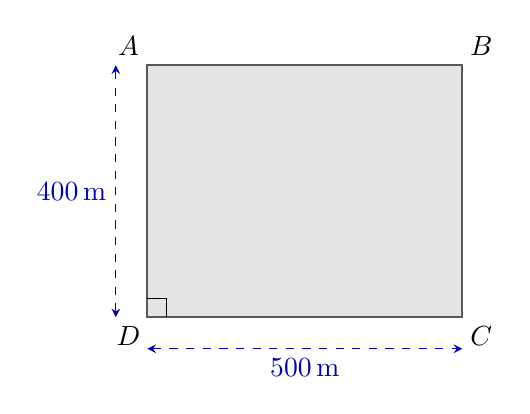
\begin{tikzpicture}[scale=0.8, >=stealth]
        % 绘制带背景色的矩形，颜色按要求改为灰色
        \draw[thick, fill=gray!20, draw=gray!70!black] (0,0) rectangle (5,4);
        
        % 标注边长
        \draw[<->, dashed, blue!70!black] (0,-0.5) -- (5,-0.5) node[midway, below] {$500 \, \mathrm{m}$};
        \draw[<->, dashed, blue!70!black] (-0.5,0) -- (-0.5,4) node[midway, left] {$400 \, \mathrm{m}$};
        
        % 顶点直角符号标注
        \draw (0.3,0) -- (0.3,0.3) -- (0,0.3);
        
        % 顶点字母 (增加学术感)
        \node at (-0.3, 4.3) {$A$};
        \node at (5.3, 4.3) {$B$};
        \node at (5.3, -0.3) {$C$};
        \node at (-0.3, -0.3) {$D$};
    \end{tikzpicture}
    \end{center}

    \begin{choices}
        \item $0.2 \, \mathrm{km}^2$
        \item $2 \, \mathrm{km}^2$
        \item $20 \, \mathrm{km}^2$
        \item $200000 \, \mathrm{km}^2$
    \end{choices}
\end{question}

\begin{solution}
    矩形场地长 $500\text{ m}$，宽 $400\text{ m}$，求面积（以 $\text{km}^2$ 表示）。\\
    先求出以平方米为单位的面积，再除以进率 $1000000$ 换算为平方千米。
    \begin{align*}
        S &= 500 \times 400 = 200000 \ \text{m}^2 \\
        S &= \frac{200000}{1000000} = 0.2 \ \text{km}^2
    \end{align*}
    故选 A。
\end{solution}

\newpage

%region 范围：初中/高中几何 - 风筝形（鸢形）性质 | 考点：邻边相等四边形的对角相等性质、四边形内角和 | 难度：中等
% 注：本题 TikZ 需要 \usetikzlibrary{quotes,angles}
\begin{question}
    如下图所示，四边形 $ABCD$ 为风筝形，其中 $AB = AD$，$CB = CD$
    已知 $\angle BAD = 90°$，$\angle BCD = 60°$，求 $\angle ABC$ 的值。
\begin{center}
        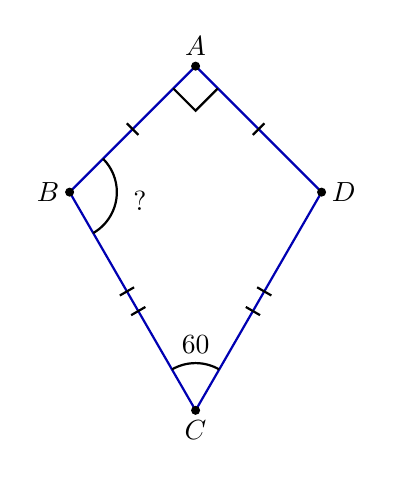
\begin{tikzpicture}[scale=0.8, >=stealth, thick]
        \coordinate (A) at (0, 2);
        \coordinate (B) at (-2, 0);
        \coordinate (C) at (0, -3.464);
        \coordinate (D) at (2, 0);

        \draw[thick, blue!70!black] (A) -- (B) -- (C) -- (D) -- cycle;

        % 单撇：AB、AD 等长标记
        \draw (-1.092,1.092) -- (-0.908,0.908);
        \draw (0.908,0.908) -- (1.092,1.092);

        % 双撇：CB、CD 等长标记
        \draw (-0.797,-1.823) -- (-1.023,-1.953);
        \draw (-0.977,-1.511) -- (-1.203,-1.641);
        \draw (1.023,-1.953) -- (0.797,-1.823);
        \draw (1.203,-1.641) -- (0.977,-1.511);

        \pic [draw, angle radius=4mm] {right angle = D--A--B};
        \pic [draw, "$60°$", angle eccentricity=1.4, angle radius=6mm] {angle = D--C--B};
        \pic [draw, "?", angle eccentricity=1.5, angle radius=6mm] {angle = C--B--A};

        \filldraw (A) circle (1.5pt) node[above] {$A$};
        \filldraw (B) circle (1.5pt) node[left] {$B$};
        \filldraw (C) circle (1.5pt) node[below] {$C$};
        \filldraw (D) circle (1.5pt) node[right] {$D$};
    \end{tikzpicture} \paren[B]
\end{center}

    \begin{choices}
        \item $75°$
        \item $105°$
        \item $135°$
        \item $210°$
    \end{choices}
\end{question}

\begin{solution}
    风筝形 $ABCD$ 中 $AB=AD$，$CB=CD$，$\angle BAD=90°$，$\angle BCD=60°$，求 $\angle ABC$。\\
    邻边相等的风筝形中，被夹在两组不等边之间的对角相等，即 $\angle ABC=\angle ADC$，设为 $x$，再用四边形内角和求解。
    \begin{align*}
        90° + 60° + 2x &= 360° \\
        2x &= 210° \\
        x &= 105°
    \end{align*}
    故选 B。
\end{solution}

%endregion



%region 范围：初中数学/初等几何 | 考点：矩形性质、弧长计算、组合图形周长 | 难度：中等
\begin{question}
    如下图所示，在矩形 $ABCD$ 中，已知 $AB=4$，$BC=6$。以点 $A$ 为圆心，以矩形的短边 $AB$ 长为半径作 $\dfrac{1}{4}$ 圆弧，交 $AD$ 于点 $E$。求图中阴影部分的周长。（取 $\displaystyle \pi = \frac{22}{7}$） \paren[B]
    
    \begin{center}
    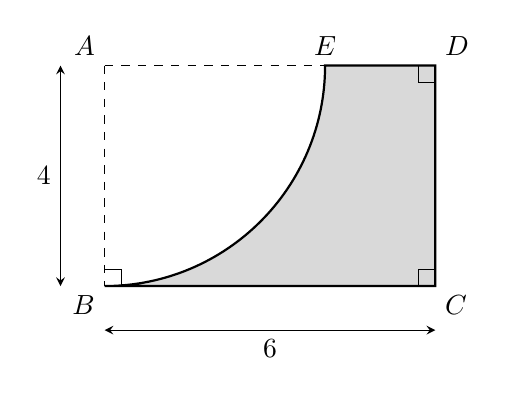
\begin{tikzpicture}[scale=0.7, >=stealth]
        % 变量定义
        \def\AB{4} % 短边
        \def\BC{6} % 长边
        
        % 顶点坐标
        \coordinate (A) at (0,\AB);
        \coordinate (B) at (0,0);
        \coordinate (C) at (\BC,0);
        \coordinate (D) at (\BC,\AB);
        \coordinate (E) at (\AB,\AB);
        
        % 绘制阴影区域 (矩形减去扇形 ABE)
        \draw[thick, fill=gray!30] (0,0) -- (\BC,0) -- (\BC,\AB) -- (\AB,\AB) arc (0:-90:\AB) -- cycle;
        
        % 绘制矩形剩余边界（无阴影部分）
        \draw[dashed, thin] (0,\AB) -- (\AB,\AB);
        \draw[dashed, thin] (0,\AB) -- (0,0);
        
        % 标注顶点
        \node[above left] at (A) {$A$};
        \node[below left] at (B) {$B$};
        \node[below right] at (C) {$C$};
        \node[above right] at (D) {$D$};
        \node[above] at (E) {$E$};
        
        % 标注边长
        \draw[<->] (-0.8, 0) -- (-0.8, \AB) node[midway, left] {$4$};
        \draw[<->] (0, -0.8) -- (\BC, -0.8) node[midway, below] {$6$};
        
        % 标注直角
        \draw (0, 0.3) -- (0.3, 0.3) -- (0.3, 0);
        \draw (\BC-0.3, 0) -- (\BC-0.3, 0.3) -- (\BC, 0.3);
        \draw (\BC, \AB-0.3) -- (\BC-0.3, \AB-0.3) -- (\BC-0.3, \AB);
        
    \end{tikzpicture}
    \end{center}

    \begin{choices}
        \item $\displaystyle \frac{100}{7}$
        \item $\displaystyle \frac{128}{7}$
        \item $\displaystyle \frac{142}{7}$
        \item $\displaystyle \frac{156}{7}$
    \end{choices}
\end{question}

\begin{solution}
    矩形 $ABCD$ 中 $AB=4$，$BC=6$，以 $A$ 为圆心 $AB$ 为半径作 $\frac{1}{4}$ 圆弧交 $AD$ 于 $E$，求阴影部分周长（$\pi=\frac{22}{7}$）。\\
    阴影边界由 $BC$、$CD$、$DE$ 三条线段及弧 $\wideparen{BE}$ 组成，逐项求长度后相加。
    \begin{align*}
        DE &= AD - AE = 6 - 4 = 2 \\
        l_{\wideparen{BE}} &= \frac{1}{4}\times2\pi R = \frac{1}{2}\times\frac{22}{7}\times4 = \frac{44}{7} \\
        C &= BC+CD+DE+l_{\wideparen{BE}} = 6+4+2+\frac{44}{7} = \frac{128}{7}
    \end{align*}
    故选 B。
\end{solution}
%endregion



%region 范围：初中数学/初等几何 | 考点：扇形面积公式及其逆运算 | 难度：中等
\begin{question}
    如下图所示，以O为圆心的扇形 $AOB$ 的圆心角 $\angle AOB = 120^\circ$。已知该扇形的面积为 $12\pi$，求扇形的半径。 \paren[B]
    
    \begin{center}
    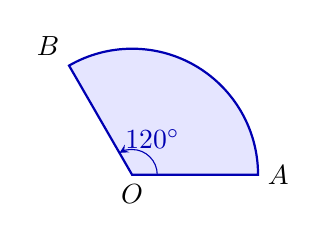
\begin{tikzpicture}[scale=0.8, >=stealth]
        % 绘制扇形并填充背景色
        \draw[thick, fill=blue!10, draw=blue!70!black] (0,0) -- (0:2) arc (0:120:2) -- cycle;
        
        % 绘制圆心角标记
        \draw[->, blue!70!black] (0.4,0) arc (0:120:0.4);
        \node[blue!70!black] at (60:0.65) {$120^\circ$};
        
        % 标注顶点字母
        \node[below] at (0,0) {$O$};
        \node[right] at (2,0) {$A$};
        \node[above left] at (120:2) {$B$};
        
        % % 标注半径
        % \node[below] at (1,0) {$r$};
    \end{tikzpicture}
    \end{center}

    \begin{choices}
        \item $3$
        \item $6$
        \item $18$
        \item $36$
    \end{choices}
\end{question}

\begin{solution}
    已知扇形圆心角 $120°$，面积 $12\pi$，求半径 $r$。\\
    代入扇形面积公式 $S=\dfrac{n\pi r^2}{360}$，解方程求 $r$。
    \begin{align*}
        12\pi &= \frac{120\pi r^2}{360} = \frac{1}{3}\pi r^2 \\
        r^2 &= 36 \\
        r &= 6
    \end{align*}
    故选 B。
\end{solution}
%endregion

% 范围：初中代数 - 代数式求值 | 考点：整式运算、代入求值 | 难度：基础
\begin{question}
    已知 $x = -2$，$y = 3$，求代数式 $2x^2 - 3xy + y^2$ 的值。 \paren[D]
    \begin{choices}
        \item $-1$
        \item $19$
        \item $31$
        \item $35$
    \end{choices}
\end{question}

\begin{solution}
    已知 $x=-2$，$y=3$，求 $2x^2-3xy+y^2$ 的值。\\
    直接代入数值逐项计算。
    \begin{align*}
        2x^2-3xy+y^2 &= 2(-2)^2-3(-2)(3)+(3)^2 \\
        &= 8+18+9 = 35
    \end{align*}
    故选 D。
\end{solution}

% 范围：初中代数 - 乘法公式与化简 | 考点：平方差公式的逆用 | 难度：中等
\begin{question}
    化简 $(2x+3)^2 - (2x-3)^2$。 \paren[A]
    \begin{choices}
        \item $24x$
        \item $12x$
        \item $8x^2 + 18$
        \item $4x^2 - 12$
    \end{choices}
\end{question}

\begin{solution}
    化简 $(2x+3)^2-(2x-3)^2$。\\
    用平方差公式 $a^2-b^2=(a+b)(a-b)$，设 $a=2x+3$，$b=2x-3$。
    \begin{align*}
        a+b &= 4x, \quad a-b = 6 \\
        (2x+3)^2-(2x-3)^2 &= 4x\times6 = 24x
    \end{align*}
    故选 A。
\end{solution}

%region 范围：信息科学与初等代数 | 考点：二进制混合四则运算 | 难度：中等
\begin{question}
    计算 $[1101_{2} \times 11_{2}] - 1010_{2}$ 的值。 \paren[C]
    
    \begin{choices}
        \item $10111_{2}$
        \item $11011_{2}$
        \item $11101_{2}$
        \item $11111_{2}$
    \end{choices}
\end{question}

\begin{solution}
    计算 $[1101_2 \times 11_2] - 1010_2$。\\
    先做二进制乘法，再用所得结果做二进制减法。
    \[
    \begin{array}{r@{\quad}l}
    1101 & {} \\
    \times \phantom{00} 11 & {} \\
    \hline
    1101 & {} \\
    + \phantom{} 11010 & {} \\
    \hline
    100111 & {}
    \end{array}
    \]
    \[
    \begin{array}{r@{\quad}l}
    100111 & {} \\
    - \phantom{00} 1010 & {} \\
    \hline
    11101 & {}
    \end{array}
    \]
    故选 C。
\end{solution}
%endregion

%region 范围：信息科学与初等代数 | 考点：二进制与八进制的快捷转换 | 难度：中等
\begin{question}
    将二进数 $11010111_{2}$ 转换为八进数，其结果为 \paren[B]
    
    \begin{choices}
        \item $227_{8}$
        \item $327_{8}$
        \item $357_{8}$
        \item $657_{8}$
    \end{choices}
\end{question}

\begin{solution}
    将二进数 $11010111_2$ 转换为八进数。\\
    自右往左每三位一组（不足补零），逐组转为对应的八进制数字。
    \[
        \underline{011}\ \underline{010}\ \underline{111}_2
    \]
    \[
        011_2=3_8, \quad 010_2=2_8, \quad 111_2=7_8
    \]
    \[
        11010111_2 = 327_8
    \]
    故选 B。
\end{solution}
%endregion

%region 范围：初中数学 - 计数制度 | 考点：八进制转十进制 | 难度：基础
\begin{question}
    将八进数 $367_{8}$ 转换为十进数，其结果为 \paren[B]
    \begin{choices}
        \item $237$
        \item $247$
        \item $257$
        \item $367$
    \end{choices}
\end{question}

\begin{solution}
    将八进数 $367_8$ 转换为十进数。\\
    按权重展开（权重从右到左依次为 $8^0,8^1,8^2$）后求和。
    \begin{align*}
        367_8 &= 3\times8^2+6\times8^1+7\times8^0 \\
        &= 192+48+7 = 247
    \end{align*}
    故选 B。
\end{solution}
%endregion

%region 范围：初中几何 - 三角形面积 | 考点：钝角三角形面积、辨别有效数据 | 难度：中等偏难
\begin{question}
    如下图所示，$\triangle ABC$ 中 $\angle ABC$ 为钝角，$BC$ 边上的高为 $AD$（$D$ 落在 $BC$ 的延长线外）。
    已知 $BC = 12$ cm，$AD = 8$ cm，$AB = 10$ cm，求 $\triangle ABC$ 的面积。

    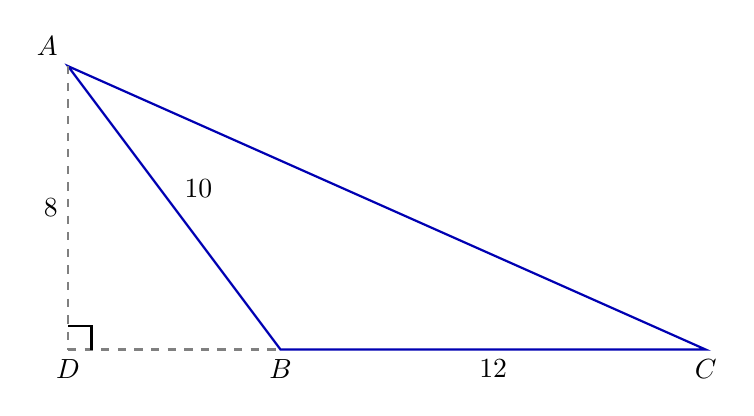
\begin{tikzpicture}[scale=0.45, >=stealth, thick]
        \coordinate (D) at (0,0);
        \coordinate (B) at (6,0);
        \coordinate (C) at (18,0);
        \coordinate (A) at (0,8);

        \draw[thick, blue!70!black] (A) -- (B) -- (C) -- cycle;
        \draw[dashed, gray] (A) -- (D);
        \draw[dashed, gray] (D) -- (B);
        \pic [draw, angle radius=3mm] {right angle = C--D--A};

        \node[above left] at (A) {$A$};
        \node[below] at (D) {$D$};
        \node[below] at (B) {$B$};
        \node[below] at (C) {$C$};

        \node[left] at ($(A)!0.5!(D)$) {$8$};
        \node[below] at ($(B)!0.5!(C)$) {$12$};
        \node[above right] at ($(A)!0.5!(B)$) {$10$};
    \end{tikzpicture} \paren[B]
    \begin{choices}
        \item $40$ cm$^2$
        \item $48$ cm$^2$
        \item $60$ cm$^2$
        \item $72$ cm$^2$
    \end{choices}
\end{question}

\begin{solution}
    $\triangle ABC$ 中 $BC=12$，$BC$ 边上的高 $AD=8$，$AB=10$，求 $\triangle ABC$ 的面积。\\
    面积只需底边及其对应的高，斜边 $AB$ 与所求公式无关，属于多余数据。
    \[
        S = \frac{1}{2}\times BC \times AD = \frac{1}{2}\times12\times8 = 48 \text{ cm}^2
    \]
    故选 B。
\end{solution}
%endregion

% 范围：初中数学 - 计数制度 | 考点：十进制转二进制 | 难度：基础
%region 范围：初中数学 - 计数制度 | 考点：十进制转二进制（除2取余法） | 难度：基础
\begin{question}
    将十进数 $45_{10}$ 转换为二进数，其结果为 \paren[B]
    \begin{choices}
        \item $100101_{2}$
        \item $101101_{2}$
        \item $101110_{2}$
        \item $110101_{2}$
    \end{choices}
\end{question}

\begin{solution}
    将十进数 $45_{10}$ 转换为二进数。\\
    用"除2取余法"反复除以 $2$ 并记录余数，最后余数由下往上排列。
    \[
        45\div2=22\cdots1,\ 22\div2=11\cdots0,\ 11\div2=5\cdots1,\ 5\div2=2\cdots1,\ 2\div2=1\cdots0,\ 1\div2=0\cdots1
    \]
    \[
        45_{10} = 101101_2
    \]
    故选 B。
\end{solution}
%endregion

\newpage
%region 范围：初中几何 - 圆与弧 | 考点：弧长公式直接应用 | 难度：基础
\begin{question}
    如下图所示，以 $O$为圆心，半径 $r = 9$ cm，圆心角 $\angle AOB = 80°$，求劣弧 $AB$ 的长度。（取 $\pi = 3.14$）
\begin{center}
        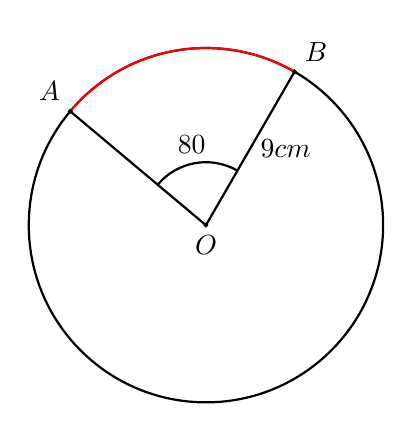
\begin{tikzpicture}[scale=0.25, >=stealth, thick]
        \coordinate (O) at (0,0);
        \coordinate (A) at (140:9);
        \coordinate (B) at (60:9);

        \draw[thick] (0,0) circle (9);
        \draw[thick] (O) -- (A);
        \draw[thick] (O) -- (B);
        \draw[thick, red] (A) arc (140:60:9);

        \filldraw (O) circle (1.5pt) node[below] {$O$};
        \filldraw (A) circle (1.5pt) node[above left] {$A$};
        \filldraw (B) circle (1.5pt) node[above right] {$B$};

        \pic [draw, "$80°$", angle eccentricity=1.3, angle radius=8mm] {angle = B--O--A};
        \node[right] at ($(O)!0.5!(B)$) {$9cm$};
    \end{tikzpicture}
\end{center}
 \paren[B]
    \begin{choices}
        \item $6.28$ cm
        \item $12.56$ cm
        \item $25.12$ cm
        \item $56.52$ cm
    \end{choices}
\end{question}

\begin{solution}
    以 $O$ 为圆心，半径 $r=9\text{cm}$，$\angle AOB=80°$，求劣弧 $AB$ 的长度（$\pi=3.14$）。\\
    代入弧长公式 $l=\dfrac{\theta}{360°}\times2\pi r$ 计算。
    \begin{align*}
        l &= \frac{80}{360}\times2\times3.14\times9 \\
        &= \frac{2}{9}\times56.52 = 12.56 \text{ cm}
    \end{align*}
    故选 B。
\end{solution}
%endregion


% %region 范围：信息科学与初等代数 | 考点：八进制转换为十进制 | 难度：基础
% \begin{question}
%     将八进制数 $356_{8}$ 转换为十进制数，其结果为 \paren[B]
    
%     \begin{choices}
%         \item $236$
%         \item $238$
%         \item $242$
%         \item $246$
%     \end{choices}
% \end{question}

% \begin{solution}
%     \textbf{解析：} \\
%     步骤 1：理解进位计数制中的按权展开法。\\
%     八进制数是以 $8$ 为底数的计数制度，从右往左数，各位的权重依次为 $8^0, 8^1, 8^2, \dots$
    
%     步骤 2：对八进制数 $356_{8}$ 进行按权展开求和：
%     \[ \displaystyle 356_{8} = 3 \times 8^2 + 5 \times 8^1 + 6 \times 8^0 \]
%     \[ \displaystyle = 3 \times 64 + 5 \times 8 + 6 \times 1 \]
%     \[ \displaystyle = 192 + 40 + 6 = 238 \]
%     因此，八进制数 $356_{8}$ 对应的十进制数为 $238$。

%     步骤 3：干扰项分析。\\
%     选项 A（$236$）的错误在于将个位数权值误算或最后加和时漏加了 $2$；\\
%     选项 C（$242$）和选项 D（$246$）通常是因为将 $8^2$ 错误地口算为 $66$ 或 $68$ 产生的计算失误。\\
    
%     故选 B。
% \end{solution}
% %endregion

%region
% 范围：初中代数 - 一元一次方程应用题 | 考点：年龄问题、列方程解应用题 | 难度：中等
% \begin{question}
%     父亲现年 $40$ 岁，儿子现年 $10$ 岁。几年后，父亲的年龄将是儿子年龄的 $3$ 倍？ \paren[A]
%     \begin{choices}
%         \item $5$ 年后
%         \item $10$ 年后
%         \item $15$ 年后
%         \item $20$ 年后
%     \end{choices}
% \end{question}

% \begin{solution}
%     \textbf{解析：} \\
%     设 $x$ 年后父亲的年龄是儿子的 $3$ 倍，则：
%     \[ \displaystyle 40 + x = 3(10 + x) \]
%     展开并移项：
%     \[ \displaystyle 40 + x = 30 + 3x \implies 40 - 30 = 3x - x \implies 10 = 2x \implies x = 5 \]
%     检验：$5$ 年后，父 $45$ 岁，子 $15$ 岁，$45 = 3 \times 15$，符合题意。 \\
%     逐一排除干扰项：
%     \begin{itemize}
%         \item[B.] $10$——列式时漏掉儿子年龄中的未知数 $x$（误设 $40+x=3\times10$），导致结果偏大。
%         \item[C.] $15$——移项或合并同类项时把系数 $2$ 误算成 $1$，运算错误所致。
%         \item[D.] $20$——把方程中 "$3$ 倍" 误理解为父亲比儿子大 $3$ 倍的差值直接计算，概念混淆导致的错误结果。
%     \end{itemize}
%     故选 A。
% \end{solution}

% % 范围：初中代数 - 二元一次方程组应用题 | 考点：数字问题、十位与个位关系 | 难度：中等偏难
% \begin{question}
%     一个两位数，十位数字与个位数字之和为 $11$。若将十位数字与个位数字对调，
%     所得新两位数比原两位数大 $63$，求原两位数。 \paren[B]
%     \begin{choices}
%         \item $20$
%         \item $29$
%         \item $38$
%         \item $92$
%     \end{choices}
% \end{question}

% \begin{solution}
%     \textbf{解析：} \\
%     设原两位数的十位数字为 $x$，则个位数字为 $(11-x)$。 \\
%     原两位数为：
%     \[ \displaystyle 10x + (11-x) = 9x + 11 \]
%     对调后的新两位数为：
%     \[ \displaystyle 10(11-x) + x = 110 - 9x \]
%     根据题意，新数比原数大 $63$：
%     \[ \displaystyle (110 - 9x) - (9x + 11) = 63 \]
%     化简：
%     \[ \displaystyle 99 - 18x = 63 \implies 18x = 36 \implies x = 2 \]
%     十位数字为 $2$，个位数字为 $11 - 2 = 9$，原两位数为 $29$。 \\
%     检验：对调后为 $92$，$92 - 29 = 63$，符合题意。 \\
%     逐一排除干扰项：
%     \begin{itemize}
%         \item[D.] $92$——把"对调后的新数"误当作题目所求的"原数"，问题理解方向搞反。
%         \item[C.] $38$——求出十位数字 $x=2$ 后，个位数字计算错误（误算成 $11-2=8$ 而非 $9$）。
%         \item[A.] $20$——只求出十位数字 $x=2$ 便直接作答，漏加个位数字 $9$。
%     \end{itemize}
%     故选 B。
% \end{solution}

% % 范围：初中代数 - 一元一次方程（分式方程）| 考点：去分母解方程 | 难度：中等
% \begin{question}
%     解方程 $\dfrac{2x-1}{3} - \dfrac{x+1}{2} = 1$，求 $x$ 的值。 \paren[D]
%     \begin{choices}
%         \item $1$
%         \item $6$
%         \item $7$
%         \item $11$
%     \end{choices}
% \end{question}

% \begin{solution}
%     \textbf{解析：} \\
%     方程两边同乘以最小公倍数 $6$，去分母：
%     \[ \displaystyle 6 \times \frac{2x-1}{3} - 6 \times \frac{x+1}{2} = 6 \times 1 \]
%     \[ \displaystyle 2(2x-1) - 3(x+1) = 6 \]
%     展开：
%     \[ \displaystyle 4x - 2 - 3x - 3 = 6 \]
%     合并同类项：
%     \[ \displaystyle x - 5 = 6 \implies x = 11 \]
%     检验：$\dfrac{2(11)-1}{3} - \dfrac{11+1}{2} = \dfrac{21}{3} - \dfrac{12}{2} = 7 - 6 = 1$，符合题意。 \\
%     逐一排除干扰项：
%     \begin{itemize}
%         \item[B.] $6$——去分母时只处理了左边两个分式，右边的常数 $1$ 忘记同乘 $6$，方程变为 $x-5=1$。
%         \item[A.] $1$——移项时符号出错，把 $x-5=6$ 误算成 $x=6-5$，减法与加法混淆。
%         \item[C.] $7$——展开 $-3(x+1)$ 时漏看括号内 $-2$ 的负号，误将 $4x-2-3x-3$ 算成 $4x+2-3x-3$。
%     \end{itemize}
%     故选 D。
%\end{solution}

%endregion 



\vfill % 与上方内容保持距离

\noindent
\newlength{\sigwidth}
\settowidth{\sigwidth}{（\hspace{4em}师）}

\begin{tabular*}{\textwidth}{@{\extracolsep{\fill}} l l l}
    出题： & 审题： & 审核： \\[4em]
    \rule{\sigwidth}{0.5pt} &
    \rule{\sigwidth}{0.5pt} &
    \rule{\sigwidth}{0.5pt} \\
    （\hspace{0em} \setterteacher ） &
    （\hspace{0em} \reviewteacher ） &
    （\hspace{0em} \auditteacher ） \\
\end{tabular*}


\newpage

\begin{center}
\textbf{参考答案}

\begin{tikzpicture}
  \pgfmathtruncatemacro{\cols}{ifthenelse(\answerkeytotal<=16,8,10)}
  \pgfmathsetlengthmacro{\boxw}{(\linewidth-0.4pt)/\cols}
  \pgfmathsetlengthmacro{\boxh}{1.2cm}
  \pgfmathsetlengthmacro{\offset}{0.15cm}

  \answerkeyitems
\end{tikzpicture}
\end{center}

\end{document}